\documentclass[12pt,french,oneside]{report}
%%%%%%%%%%%%%%%%%%%%%%%%%%%%%%%%%%%%%%%%%%%%%%%%%%%%%%%%%%%%%%%%%%%%%%%%%%%%%%%
\input{preambule_lua_2016}
%%%%%%%%%%%%%%%%%%%%%%%%%%%%%%%%%%%%%%%%%%%%%%%%%%%%%%%%%%%%%%%%%%%%%%%%%%%%%%%

%%%%%%%%%%%%%%%%%%%%%%%%%%%%%%%%%%%%%%%%%%%%%%%%%%%%%%%%%%%%%%%%%%%%%%%%%%%%%%%%%%%%%%
%entête bac blanc
\newcommand{\bacblanc}{
\thispagestyle{empty}


\includegraphics[scale=0.3]{logo_academie} \hfill 

\includegraphics[scale=0.2]{logo_augustin_thierry}
\normalsize

\vspace*{24pt}

\hrule

\vspace*{24pt}
\begin{center}
\color{gray}
\LARGE
\begin{bf}
DEVOIR COMMUN\\
\vspace{1cm}
de\\
\vspace{1cm}
\Huge
\textcolor{black}{MATH\'EMATIQUES}\\
\LARGE
\vspace{1cm}
Mercredi 7 décembre\\
\vspace{1cm}
Durée : 1 heure 45 min
\end{bf}
\normalsize
\color{black}
\end{center}

\vspace*{24pt}


\hrulefill


\vspace*{24pt}


\large
\begin{itemize}
\item[$\star$] L'usage de la calculatrice est autorisé.

\item[$\star$] \emph{L'ensemble du sujet} est à rendre avec la copie.

\item[$\star$] \textbf{Inscrivez votre \emph{nom, prénom et classe} en haut de chaque page de l'énoncé.}
\end{itemize}

\centrer{Ce sujet comporte \pageref{LastPage} pages dont la page de garde}
\normalsize
\newpage
}
%%%%%%%%%%%%%%%%%%%%%%%%%%%%%%%%%%%%%%%%%%%%%%%%%%%%%%%%%%%%%%%%%%%%%%%%%%%%%%%
\setmainfont{Arial}
%%%%%%%%%%%%%%%%%%%%%%%
%% DEBUT DU DOCUMENT %%
%%%%%%%%%%%%%%%%%%%%%%%

\begin{document}

\setlength\parindent{0mm}
\bacblanc 		%entête bac blanc

\renewcommand \footrulewidth{0.2pt}%
\renewcommand \headrulewidth{0.2pt}%
\pagestyle{fancy}
\fancyhead{Nom, Prénom :\dotfill Classe : 2nde\dots\dots
\vspace{6pt}}
\pieddepage{2nde}{\thepage / \pageref{LastPage}}{Année 2016-2017}

%%%%%%%%%%%%%%%%%%%%%%%Page 1%%%%%%%%%%%%%%%%%%%%%%%%%%%%%%%%%%%%%%%%
\begin{spacing}{1.2}
%%%%%%%%%%%%%%%%%%%%%%%%%%%%%%%%%%%%%%%%%%%%%%%%%%%%%%%%%%%%
%%%%%%%%%%%%%%%%%%%%%%%%%%%%%%%%%%%%%%%%%%%%%%%%%%%%%%%%%%%%%%%%%%%%%%%%%
%%%%%%%%%%%%%%%%%%%%%%%% exercice 1 %%%%%%%%%%%%%%%%%%%%%%%%%%%%%%%%%%%%%
%%%%%%%%%%%%%%%%%%%%%%%%%%%%%%%%%%%%%%%%%%%%%%%%%%%%%%%%%%%%%%%%%%%%%%%%%
\begin{Exercice}[(10,5 points)]%

\begin{center}
\textit{Dans tout l'exercice, on utilise le mot " masse " qui est souvent remplacé par " poids " dans ce genre de contexte dans le langage courant.}
\end{center}

L'un des matchs de quart de finale de la coupe du monde de Rugby 2015, a vu s'affronter la Nouvelle-Zélande et la France.

Avant ce match, un statisticien avait été chargé par l'équipe de France de réaliser une étude statistique sur les masses des deux équipes.

\textbf{Partie \rond{A} : Masses des joueurs de l'équipe de Nouvelle-Zélande}

Le tableau suivant résume les masses des 31 joueurs sélectionnés pour intégrer l'équipe de Nouvelle-Zélande.

\begin{center}
\begin{tabular}{|m{1.5cm}|*{9}{M{1cm}|}}
\hline
\cellcolor{blue!20}\textbf{Masses (en kg)}
&\textbf{84}
&\textbf{91}
&\textbf{95}
&\textbf{100}
&\textbf{105}
&\textbf{108}
&\textbf{112}
&\textbf{119}
&\textbf{125}\\
\hline
\cellcolor{blue!20}\textbf{Effectifs}
&2&5&2&3&4&5&5&4&1\\
\hline
\cellcolor{blue!20}\textbf{E.C.C.}
& & & & & & & & & \\
\hline
\end{tabular}
\end{center}

\textit{E.C.C. : Effectifs Cumulés Croissants}

\begin{enumerate}
\item Compléter le tableau précédent.

\item 	\begin{enumerate}
	\item Calculer l'étendue des masses de l'équipe de Nouvelle-Zélande.

	\item Justifier, par un calcul, que la masse moyenne de l'équipe de Nouvelle-Zélande, arrondie au kilogramme est 104 kg.
	
	\item Déterminer une masse médiane de l'équipe de Nouvelle-Zélande. 
	
	\textit{On détaillera la méthode utilisée}.
	
	\item Déterminer l'écart inter-quartile en détaillant les calculs.
	
	\end{enumerate}

\end{enumerate}

\textbf{Partie \rond{B} : Masses des joueurs de l'équipe de France}

Sur les 31 joueurs français, on ne possède que les informations suivantes :

\boldmath
\begin{center}
\begin{tabular}{|m{2cm}|*{6}{M{1.8cm}|}}
\hline
\cellcolor{blue!20}\textbf{Masses}\par \textbf{(en kg)}
&$\intervallefo{80}{90}$
&$\intervallefo{90}{100}$
&$\intervallefo{100}{110}$
&$\intervallefo{110}{120}$
&$\intervallefo{120}{130}$
&$\intervallefo{130}{160}$
\\
\hline
\cellcolor{blue!20}\textbf{Effectifs}
&5&11&4&7&3&1\\
\hline
\cellcolor{blue!20}\textbf{Fréquences}
& & & & & & \\
\hline
\cellcolor{blue!20}\textbf{F.C.C.}
& & & & & & \\
\hline
\end{tabular}
\end{center}
\unboldmath

\textit{F.C.C. : Fréquences Cumulées Croissantes}

\begin{enumerate}
\item Compléter le tableau précédent (\textit{On arrondira au centième}).

\item 	\begin{enumerate}[label=\alph*)]
	\item En détaillant les calculs, déterminer une valeur approchée de la masse moyenne des joueurs de l'équipe de France (\textit{On arrondira le résultat au kilogramme}).
	
	\item On a représenté ci-dessous le polygone des fréquences cumulées croissantes. 
	
	Avec la précision permise par le graphique, déterminer une masse médiane et les quartiles $Q_1$ et $Q_3$ des masses des joueurs de l'équipe de France. \textit{(On fera apparaître les traits de lecture sur le graphique).}

	\end{enumerate}

\end{enumerate}

\begin{center}
\begin{tikzpicture}[xscale=1.5,yscale=0.8,>=stealth]
\tkzInit[xmin=80,xmax=160,xstep=10,ymax=1.1,ystep=0.1]
\tkzGrid
\tkzDrawX[line width=1.5pt,color=blue,below right,label=Poids,>=stealth]
\tkzLabelX%[label options={below=12pt,rotate=-45}]
\tkzDrawY[line width=1.5pt,color=blue,above left,label=F.C.C.,>=stealth]
\tkzLabelY%[label options={left=6pt}]
\tkzDefPoint(80,0){A}
\tkzDefPoint(90,0.161){B}
\tkzDefPoint(100.94,0.516){C}
\tkzDefPoint(110,0.645){D}
\tkzDefPoint(120,0.871){E}
\tkzDefPoint(130,0.968){F}
\tkzDefPoint(160,1){G}
\tkzDrawSegments[color=red,line width=1.5pt](A,B B,C C,D D,E E,F F,G)
\tkzDrawPoints[shape=rectangle,color=red,size=4pt](B,C,D,E,F,G)
%Médiane
%\tkzDefPoint(14.9,250){L}
%\tkzDefPoint(14.9874,250){M}
%\tkzDefPoint(14.9874,0){N}
%\tkzDrawSegment[color=OliveGreen,line width=1.5pt,style=dashed](L,M)
%\tkzDrawSegment[->,>=stealth,color=OliveGreen,line width=1.5pt,style=dashed](M,N)
%\tkzText[below=30pt,color=OliveGreen](N){Med}
%1er quartile
%\tkzDefPoint(14.9,125){R}
%\tkzDefPoint(14.9639,125){S}
%\tkzDefPoint(14.9639,0){T}
%\tkzDrawSegment[color=OliveGreen,line width=1.5pt,style=dashed](R,S)
%\tkzDrawSegment[->,>=stealth,color=OliveGreen,line width=1.5pt,style=dashed](S,T)
%\tkzText[below=30pt,color=OliveGreen](T){$Q_1$}
%3eme quartile
%\tkzDefPoint(14.9,375){U}
%\tkzDefPoint(15.009,375){V}
%\tkzDefPoint(15.009,0){W}
%\tkzDrawSegment[color=OliveGreen,line width=1.5pt,style=dashed](U,V)
%\tkzDrawSegment[->,>=stealth,color=OliveGreen,line width=1.5pt,style=dashed](V,W)
%\tkzText[below=30pt,color=OliveGreen](W){$Q_3$}
\end{tikzpicture}
\end{center}

\textbf{Partie \rond{C} : Interprétation des résultats}

\begin{center}
\textit{Les résultats suivants seront tous justifiés. On s'appuiera sur les caractéristiques de position et/ou de dispersion des parties \rond{A} et \rond{B} lorsque cela sera nécessaire.}
\end{center}

\begin{enumerate}

\item %Si l'on considère que la force d'un joueur de rugby est uniquement liée à sa masse, y-a-t'il un joueur de l'équipe de France qui puisse rivaliser quel que soit le joueur Néo-Zélandais engagé en face ?
Interpréter la fréquence cumulée croissante de la classe $\intervallefo{110}{120}$ obtenue dans le tableau des masses des joueurs de l'équipe de France.

\item %Sachant qu'une équipe de Rugby est composée de 15 joueurs seulement. L'équipe de France peut-elle avoir une équipe composée de joueurs pesant tous au moins 95 kg ?
Quelle est le pourcentage des joueurs de l'équipe de France dont la masse est au moins de 100 kg ?

\item Chaque entraîneur des deux équipes souhaite avoir 31 joueurs dont les masses sont les plus homogènes possibles. Lequel des entraîneurs a l'équipe correspondant le mieux à ce critère ?


\end{enumerate}


\end{Exercice}

%%%%%%%%%%%%%%%%%%%%%%%%%%%%%%%%%%%%%%%%%%%%%%%%%%%%%%%%%%%%%%%%%%%%%%%%%
%%%%%%%%%%%%%%%%%%%%%%%% exercice 2 %%%%%%%%%%%%%%%%%%%%%%%%%%%%%%%%%%%%%
%%%%%%%%%%%%%%%%%%%%%%%%%%%%%%%%%%%%%%%%%%%%%%%%%%%%%%%%%%%%%%%%%%%%%%%%%
%\newpage
\bigskip
\begin{Exercice}[(7,5 points)]%

\medskip

On se place dans un repère orthonormé \OIJ. 

%On complètera, au fur et à mesure, la figure ci-dessus.



\begin{enumerate}
\item Placer, dans le repère ci-dessous, les points A, B, C de coordonnées $A(-2\pv 3)$, $B(2\pv 1)$, $C(0\pv -3)$.

\begin{center}
\begin{tikzpicture}[scale=1]
\tkzInit[xmin=-6,xmax=5,ymin=-6,ymax=5]
\tkzGrid[sub,subxstep=0.5,subystep=0.5]
\tkzDrawXY[>=stealth,color=blue,line width=1.5pt,label=]
\tkzClip

%Points de la figure
%\tkzDefPoint(-2,3){A}
%\tkzDefPoint(2,1){B}
%\tkzDefPoint(0,-3){C}
%\tkzDrawPoints[size=2,color=red](A,B,C)

%Repère
\tkzDefPoint(0,0){O}
\tkzDefPoint(1,0){I}
\tkzDefPoint(0,1){J}
\tkzLabelPoints[below left=3pt,font=\boldmath,color=red](O)
\tkzLabelPoints[below right=3pt,font=\boldmath,color=red](I)
\tkzLabelPoints[above left=3pt,font=\boldmath,color=red](J)
\tkzDrawPoints[shape=cross out,color=red,size=3pt](O,I,J)
\end{tikzpicture}
\end{center}

\item Calculer les coordonnées de K, milieu du segment [AC].

%\color{blue}
\item 	\begin{enumerate}
	\item Calculer la longueur AC.
	\end{enumerate}
	
	\textit{Pour la suite, on donne $AB=\sqrt{20}$ et $BC=2\sqrt{5}$.}
	
	\begin{enumerate}[start=2]
	\item Le triangle ABC est-il isocèle ? Justifier.
	
	\item Le triangle ABC est-il rectangle ? Justifier.
	
	\end{enumerate}
%\color{black}
\item Soit D le symétrique de B par rapport à K . 

\begin{enumerate}
\item Justifier que ABCD est un parallélogramme.

\item Calculer les coordonnées de D.

\end{enumerate}

\item %\sout{Que peut-on dire du parallélogramme ABCD ?} 
Le parallélogramme ABCD est-il un parallélogramme particulier ?

Justifier à l'aide des questions précédentes.

%\item Soit M un point de coordonnées $M(6\pv y)$, où $y$ est un réel quelconque.
%
%Déterminer les valeurs de $y$ pour que $AM=10$.

\end{enumerate}

\end{Exercice}



%%%%%%%%%%%%%%%%%%%%%%%%%%%%%%%%%%%%%%%%%%%%%%%%%%%%%%%%%%%%%%%%%%%%%%%%%
%%%%%%%%%%%%%%%%%%%%%%%% exercice 3 %%%%%%%%%%%%%%%%%%%%%%%%%%%%%%%%%%%%%
%%%%%%%%%%%%%%%%%%%%%%%%%%%%%%%%%%%%%%%%%%%%%%%%%%%%%%%%%%%%%%%%%%%%%%%%%

%\newpage
\bigskip
\begin{Exercice}[(2,5 points)]%

Voici trois algorithmes.

\bigskip

\begin{minipage}{0.33\linewidth}
\begin{center}
\textbf{Algorithme 1}

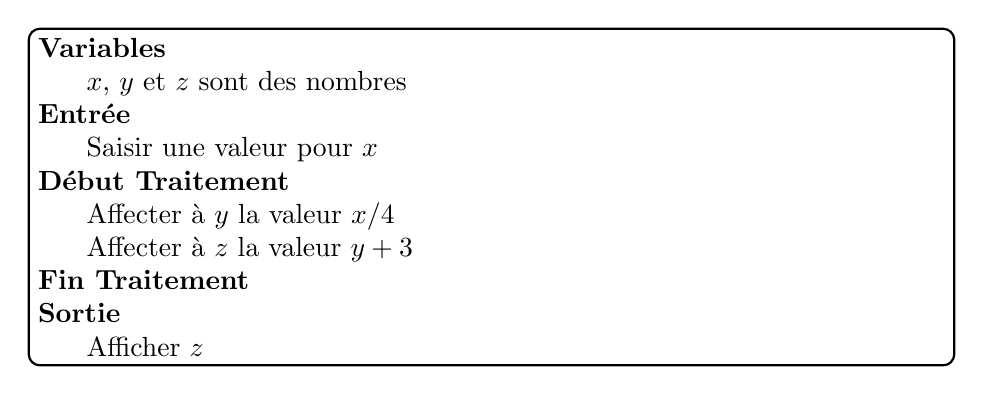
\begin{tikzpicture}
\node[rectangle,draw=black,rounded corners,thick,fill=white]{%
\begin{minipage}{0.95\linewidth}
\textbf{Variables} \\
\hspace*{0.5cm} $x$, $y$ et $z$ sont des nombres \\
\textbf{Entrée} \\
\hspace*{0.5cm} Saisir une valeur pour $x$\\
\textbf{Début Traitement} \\
\hspace*{0.5cm} Affecter à $y$ la valeur $x/4$\\
\hspace*{0.5cm} Affecter à $z$ la valeur $y+3$\\
\textbf{Fin Traitement} \\
\textbf{Sortie} \\
\hspace*{0.5cm} Afficher $z$
\end{minipage}
};\end{tikzpicture}
\end{center}
\end{minipage}
\hfill
\begin{minipage}{0.33\linewidth}
\begin{center}
\textbf{Algorithme 2}

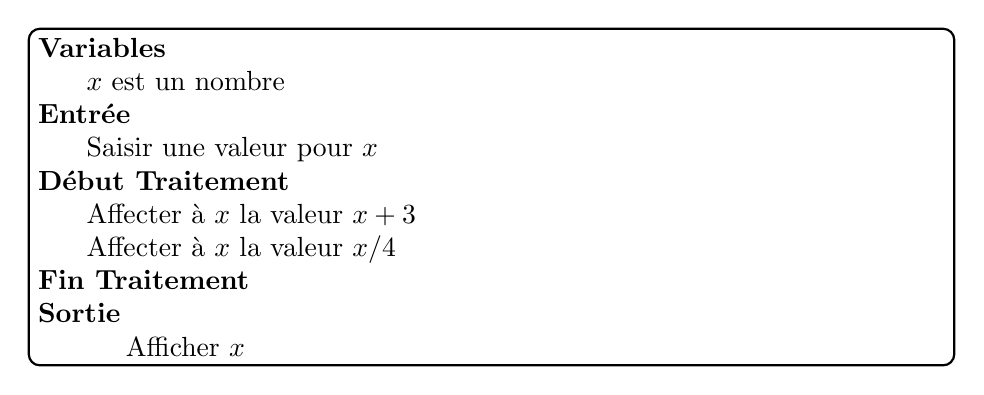
\begin{tikzpicture}
\node[rectangle,draw=black,rounded corners,thick,fill=white]{%
\begin{minipage}{0.95\linewidth}
\textbf{Variables} \\
      \hspace*{0.5cm} $x$ est un nombre\\
\textbf{Entrée} \\
      \hspace*{0.5cm} Saisir une valeur pour $x$\\
\textbf{Début Traitement} \\
      \hspace*{0.5cm} Affecter à $x$ la valeur $x+3$\\
      \hspace*{0.5cm} Affecter à $x$ la valeur $x/4$\\
\textbf{Fin Traitement} \\
\textbf{Sortie} \\
      \hspace*{1cm} Afficher $x$
\end{minipage}
};\end{tikzpicture}
\end{center}
\end{minipage}
\hfill
\begin{minipage}{0.33\linewidth}
\begin{center}
\textbf{Algorithme 3}

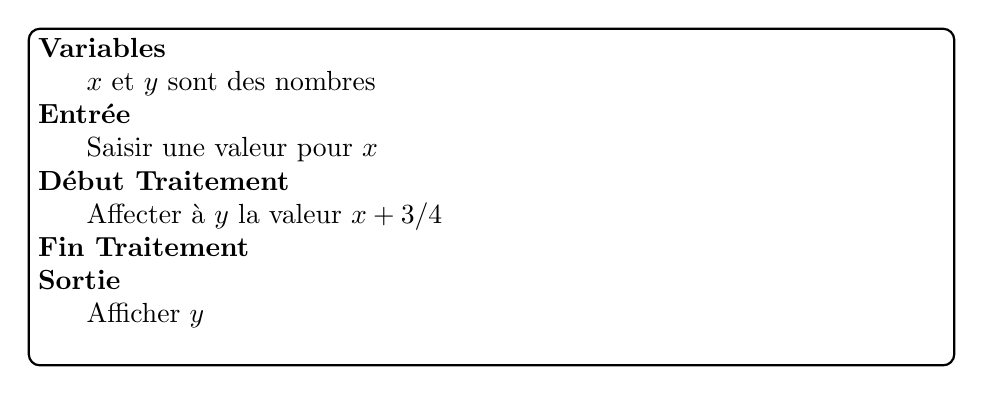
\begin{tikzpicture}
\node[rectangle,draw=black,rounded corners,thick,fill=white]{%
\begin{minipage}{0.95\linewidth}
\textbf{Variables} \\
      \hspace*{0.5cm} $x$ et $y$ sont des nombres \\
\textbf{Entrée} \\
      \hspace*{0.5cm} Saisir une valeur pour $x$\\
\textbf{Début Traitement} \\
      \hspace*{0.5cm} Affecter à $y$ la valeur $x+3/4$\\
\textbf{Fin Traitement} \\
\textbf{Sortie} \\
      \hspace*{0.5cm} Afficher $y$\\
      
\end{minipage}
};\end{tikzpicture}
\end{center}
\end{minipage}

\begin{enumerate}
\item %Afficher le résultat en sortie de chaque algorithme obtenu avec $x=-4$.

%\textit{On détaillera les étapes de calcul}.
\begin{enumerate}
\item Quel résultat obtient-on en sortie de l'algorithme 1 avec $x=-4$ ? \textit{On détaillera les étapes.}

\item Obtient-on le même résultat en sortie, avec $x=-4$, avec l'algorithme 2 ? Justifier.

\end{enumerate}

\item Afin de dresser un tableau de valeurs de la fonction $f$ définie sur $\R$ par $f(x)=\dfrac{x+3}{4}$, 

on souhaite utiliser un algorithme.

Un seul des trois algorithmes précédents correspond à ce qui est attendu. Lequel est-ce ?

Justifier ce choix.

\end{enumerate}


\end{Exercice}

%%%%%%%%%%%%%%%%%%%%%%%%%%%%%%%%%%%%%%%%%%%%%%%%%%%%%%%%%%%%%%%%%%%%%%%%%
%%%%%%%%%%%%%%%%%%%%%%%% exercice 4 %%%%%%%%%%%%%%%%%%%%%%%%%%%%%%%%%%%%%
%%%%%%%%%%%%%%%%%%%%%%%%%%%%%%%%%%%%%%%%%%%%%%%%%%%%%%%%%%%%%%%%%%%%%%%%%
%\newpage
\bigskip
\begin{Exercice}[(9,5 points)]%

La courbe $\mathcal{C}_f$ suivante est la courbe représentative d'une fonction $f$.

\begin{center}
\begin{tikzpicture}[scale=1.2]
\tkzInit[xmin=-3,xmax=10,ymin=-1.5,ymax=6]
\tkzGrid[sub,subxstep=0.1,subystep=0.1]
%\tkzAxeXY
\tkzDrawX[line width=2pt,color=blue,below right,>=stealth]%,label=Rang année]
\tkzLabelX%[label options={below=12pt,rotate=-45}]
\tkzDrawY[line width=2pt,color=blue,above left,>=stealth]%,label=Montant (en \euro)]
\tkzLabelY[label options={left=6pt}]
\tkzClip
\boldmath 
\draw[line width=2pt,color=OliveGreen] plot[smooth=200]%,mark=+,mark options={color=black,scale =2.5}] 
coordinates{(-2,5)(-1,3)(0,2)(1,0)(2,-1)(3,0)(4,2)(5,3)(6,5)(9,3)} node[below left]{$\calig C_f$};
\tkzDrawPoints[size=2pt,color=OliveGreen]({-2,5},{9,3})
\end{tikzpicture}
\end{center}
\unboldmath 

\textbf{Partie \rond{A}}

Avec la précision permise par le graphique, répondre aux questions suivantes (\textit{On laissera les traits de lecture apparents}) :

\begin{enumerate}
\item Quel est l'ensemble de définition de la fonction $f$ ? On le notera $\mathcal{D}_f$.

\item Déterminer graphiquement :
\begin{enumerate}
\item $f(0)$.

\item L'image de 4 par $f$.

\item Les éventuels antécédents de 3 par $f$.

\end{enumerate}

\item Résoudre graphiquement, sur $\mathcal{D}_f$, les équations et inéquations suivantes :
\begin{enumerate}
\item $f(x)=2$.

\item $f(x)>0$.

\item $f(x)\leq 3$.

\end{enumerate}

\item Dresser le tableau de signes de $f(x)$ sur $\mathcal{D}_f$.
\end{enumerate}

\textbf{Partie \rond{B}}

\medskip

On considère la fonction $g$ définie sur $\intervalleff{-2}{9}$ par $g(x)=\dfrac{1}{6}x^2-x+\dfrac{1}{2}$.

\begin{enumerate}
\item Dresser un tableau de valeurs de la fonction $g$ sur $\intervalleff{-2}{9}$ avec un pas de 1. 

\textit{On arrondira à $10^{-1}$ près.}

\item Tracer la courbe représentative de la fonction $g$ dans le repère précédent.

\item Déterminer, par le calcul, l'ordonnée exacte du point A d'abscisse $\dfrac{3}{2}$ de la courbe représentative de la fonction $g$.

\item Le point B de coordonnées $\left(\sqrt{3}\pv -0,7\right)$ appartient-il à la courbe représentative de la fonction $g$ ? Justifier en détaillant les calculs.

\item Le point C de coordonnées $(-3\pv 5)$ appartient-il à la courbe représentative de la fonction $g$ ? Justifier.
\end{enumerate}

\end{Exercice}


%%%%%%%%%%%%%%%%%%%%%%%%%%%%%%%%%%%%%%%%%%%%%%%%%%%%%%%%%%%%
%%%%%%%%%%%%%%%%%%%%%%%%%%%%%%%%%%%%%%%%%%%%%%%%%%%%%%%%%%%%
\end{spacing}

%%%%%%%%%%%%%%%%%%%%%%%%%%%%%%%%%%%%%%%%%%%%%%%%%%%%%%%%%%%%
%%%%%%%%%%%%%%%%%%%%%
%% FIN DU DOCUMENT %%
%%%%%%%%%%%%%%%%%%%%%
\end{document}